\chapter{Simulering}


For at kunne sammenligne teori og praksis, kan højtaler-dataen fra tabel \ref{tab:TS} benyttes til at udformere et simuleret frekvensrespons, ud fra de forskellige portlængder på basrefleksen. 

Ved at beregne volumenhastigheden for den elektriske impedans, kan man opdele bidraget fra fronten af højtaleren, samt for porten, for til sidst at lave det samlede tryk til en ønsket afstand. 


\subsection{Volumenhastighed Front:}
\label{sec:sim_calc}

Ud fra impedansen af det samlede system, kan volumenhastigheden for højtalerenheden i kabinettet beregnes. Dette er hastigheden af det volumen af luft som skubbes foran højtaleren. 

{\Large\(qF=\)}{\huge \(\frac{F_A}{R_{AE}+s*M_{AS}+\frac{1}{s*C_{AS}}+Ras+\frac{1}{(s*C_{AB}+\frac{1}{s*M_{AP}}}}\) }

I denne beregning, indgår også \textit{massen af luften i porten} ($M_{AP})$, som beror sig på radius af porten og længden af porten:\\

\(M_{AP}=\frac{(\rho)}{S_P}*(L_P+1.46*\sqrt{\frac{S_P}{\pi}}\))

Da kabinettet i projektet allerede var konstrueret med en enkelt port, er radius af porten fastsat fra start.

\(r_P=0.025 m\)		\hspace{6.2cm} Portens Radius\\
\(S_P=\pi*r_P^2=pi*0.025^2=0.0020 m^2\)		\hspace{2cm} Portens overfladeareal\\

\(L_P=\frac{\gamma*P_0}{\rho*(2*\pi*f_p)^2*V_{B}}-1.46\sqrt{\frac{S_P}{\pi}}\)			\hspace{3cm} Hvor $\gamma \approx 1.4$ \& $P_0=100*10^3)$\\

Dermed får vi den optimale portlængde:\\

\(L_P=\frac{1.4*100*10^3}{1.18*(2*\pi*44)^2*16.5*10-3}-1.46\sqrt{\frac{0.0020}{\pi}}=15cm\)


\subsection{Volumenhastighed Port:}

Ovenpå at beregne volumenhastigheden for højtalerenheden, beregnes bidraget fra porten ud fra følgende formel:

{\Large\(qP=-qF*\)}{\huge \(\frac{\frac{1}{s*C_{AB}}}{\frac{1}{s*C_{AB}}+s*M_{AP}}\) }
\fxnote{s 61 Tores bog}


\subsection{Beregning af samlet lydtryk:}

For at omregne de to volumenhastigheder til et lydtryk i afstanden \textit{r}, benyttes følgende formel:

\(L=20*log_{10}(\frac{\frac{\rho*f}{r}*(qF+qP)}{pRef}) dB SPL\)

\section{Resultater}

Ved beregningen i Matlab, kan der simuleres et plot for frekvenskarakteristikken af bidraget fra højtalerenheden, porten og det samlede bidrag. \\

For at eftervise at det 15cm lange rør er den optimale længde for basreflexen i projektets kabinet, er der ligeledes lavet simuleringer med de to andre test-størrelser til rådighed: 7cm og 3.5cm.\\

\subsection{Kort rør - 3.5 cm}

Ved brug af en rørlængde på 3.5 cm, fås frekvensresponset som ses på figur \ref{fig:sim_kort}. \\
Det fremgår af figuren at portens resonansfrekvens fp er helt oppe på 71 Hz, hvilket er over 2/3 højere end højtalerennhedens resonans. Dermed er porten ikke ordentligt afstemt, og de 24dB/oktav koster betydeligt på de lavere frekvenser. 

\begin{figure}[h!]
	\centering
	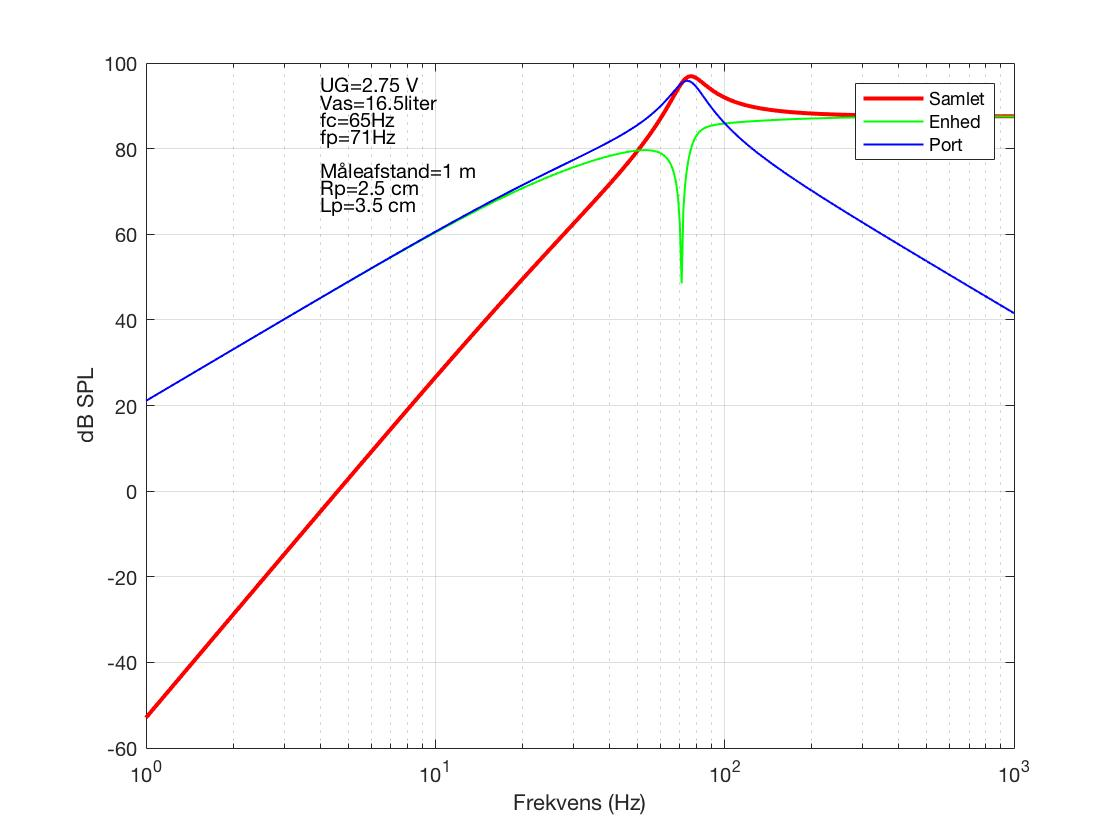
\includegraphics[width=.8\textwidth]{Pics/sim_kort}
	\caption{Simuleret frekvensrespons ved $L_P$=3.5cm } 
	\label{fig:sim_kort}
\end{figure}

\subsection{Mellemlangt rør - 7 cm}

Ved brug af en rørlængde på 7 cm, fås frekvensresponset som ses på figur \ref{fig:sim_medium}. \\
Det ses nu, at portens resonansfrekvens er rykket længere ned og nu resonerer ved 58 Hz. Dette er væsentligt tættere på at være afstemt med højtalerenhedens opgivne 45 Hz resonans, men er endnu ikke nede og give et korrekt bidrag for at løfte de lavere frekvenser. 

Det er ligeledes værd at notere, at det generelle gain som er opnået, er lavere for det mellemlange rør end for det korte rør.  

\begin{figure}[h!]
	\centering
	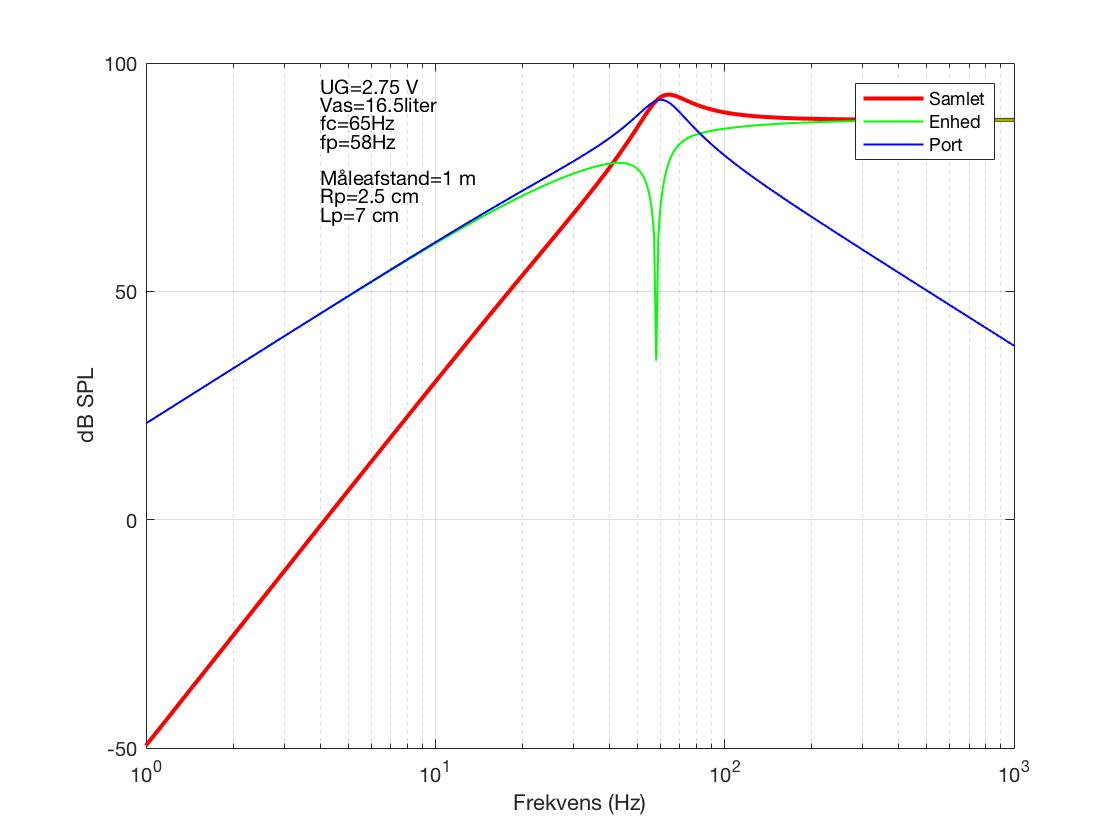
\includegraphics[width=.8\textwidth]{Pics/sim_medium}
	\caption{Simuleret frekvensrespons ved $L_P$=7cm } 
	\label{fig:sim_medium}
\end{figure}

\subsection{Langt rør - 15 cm}

Ved brug af en rørlængde på 15 cm, fås frekvensresponset som ses på figur \ref{fig:sim_langt}. \\
Denne længde er den teoretisk optimale, som det blev beregnet ovenfor i sektion \ref{sec:sim_calc}, og resonerer nu i 44 Hz, så port og højtaler er korrekt afstemt. 
Der opretholdes dermed en højere gengivelse af de lavere frekvenser end det var muligt før og teorien stammer dermed overens med simuleringen. 

\begin{figure}[h!]
	\centering
	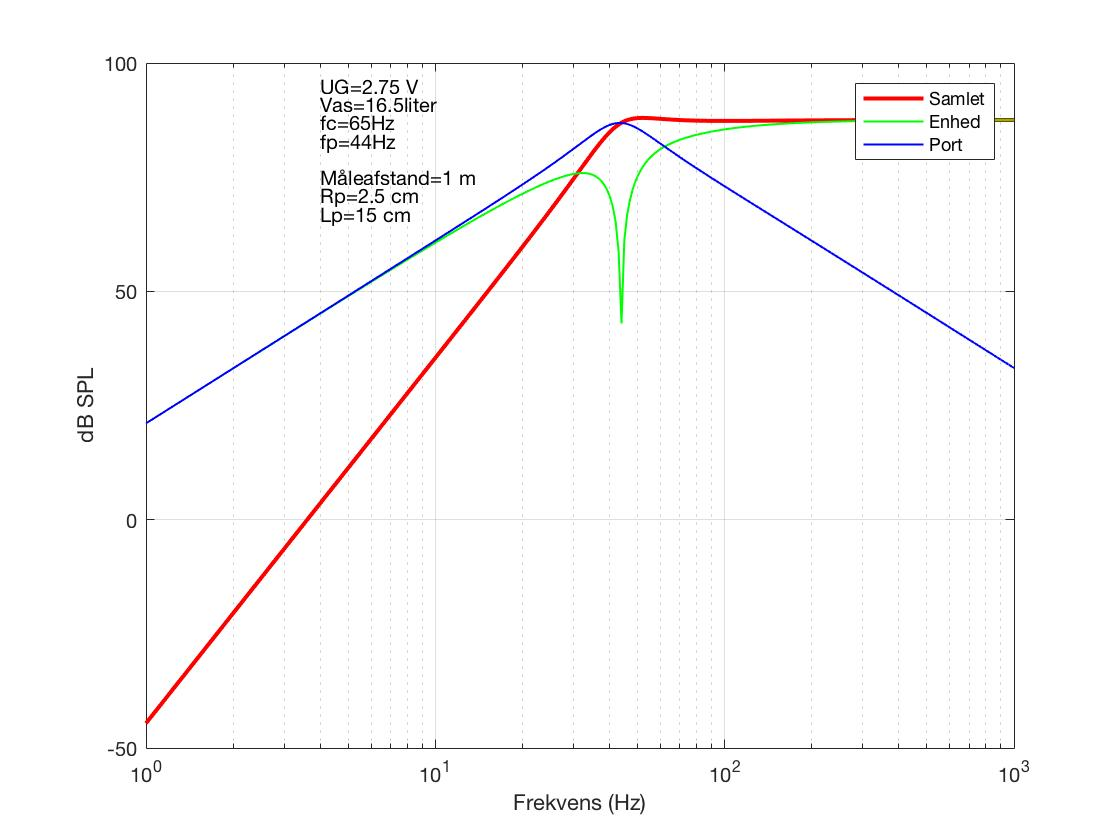
\includegraphics[width=.8\textwidth]{Pics/sim_lang}
	\caption{Simuleret frekvensrespons ved $L_P$=15cm } 
	\label{fig:sim_langt}
\end{figure}


\section{Bidrag fra reflektion}
\label{sec:reflection}
Foruden at skabe den bedst mulige gengivelse af de laveste frekvenser muligt vha. et afstemt basreflex-kabinet, fokuserer dette projekt ligeledes med at forsøge at skabe et yderligere bidrag i bassen ved hjælp af et refleksionsbidrag for nærliggende overflader. 

Teorien beror sig på et fokus for refleksion ved en højtaler placeret i en hvis højde fra gulvet, men grundet de lave frekvenser og en sfærisk udbredelse, vil dette projekt ligeledes fokusere på et bidrag ift refleksion fra vægge. 
Dette er dog et fokuspunkt for målingen, hvor simuleringen alene benytter den teori afbilledet i bogen (figur \ref{fig:reflect}
\fixme{tores bog reference}


\begin{figure}[h!]
	\centering
	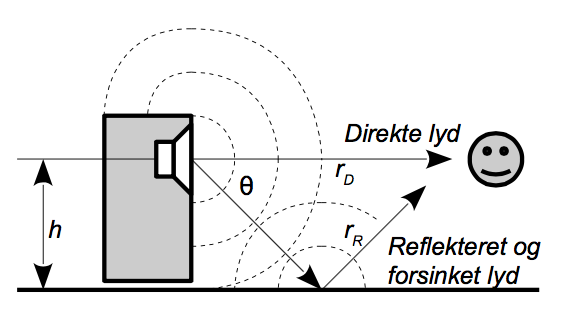
\includegraphics[width=.7\textwidth]{Pics/reflect}
	\caption{Afbilding af teorien bag reflekteret lyd (Elektro-akustik,TAS, fig 1.20) } 
	\label{fig:reflect}
\end{figure}

I jagten på et positivt bidrag i de lave frekvenser, vil man dog kunne forvente en destuktiv interferens, når højtaleren har en afstand til den reflekterede overflade på en halv bølgelængde. Herefter, vil frekvensresponset være temmeligt irregulært, før disse forstyrrelser dør ud i takt med at direktiviteten bliver mere betydende ved høje frekvenser. 

Denne frekvens, også beskrevet som det første minimum, beregnes ved:\\

\(r_R(=\sqrt{r_D^2+4h^2})\) \hspace{2cm}Den reflekterede længde\\
\(f_R=\frac{c}{2(r_R-r_D)}\)\\

Ved højtalerens øgede højder fra gulvet, kan det ses på figur \ref{fig:refleksionsbidrag} at frekvensen for det første minimum falder længere og længere ned. Så ud fra den simple betragtning af denne figur, kan det konkluderes at det må give det højeste stabile bidrag, op imod de højeste frekvenser, ved at sætte højtaleren så tæt på den reflektive overflade som muligt.

\begin{figure}[h!]
	\centering
	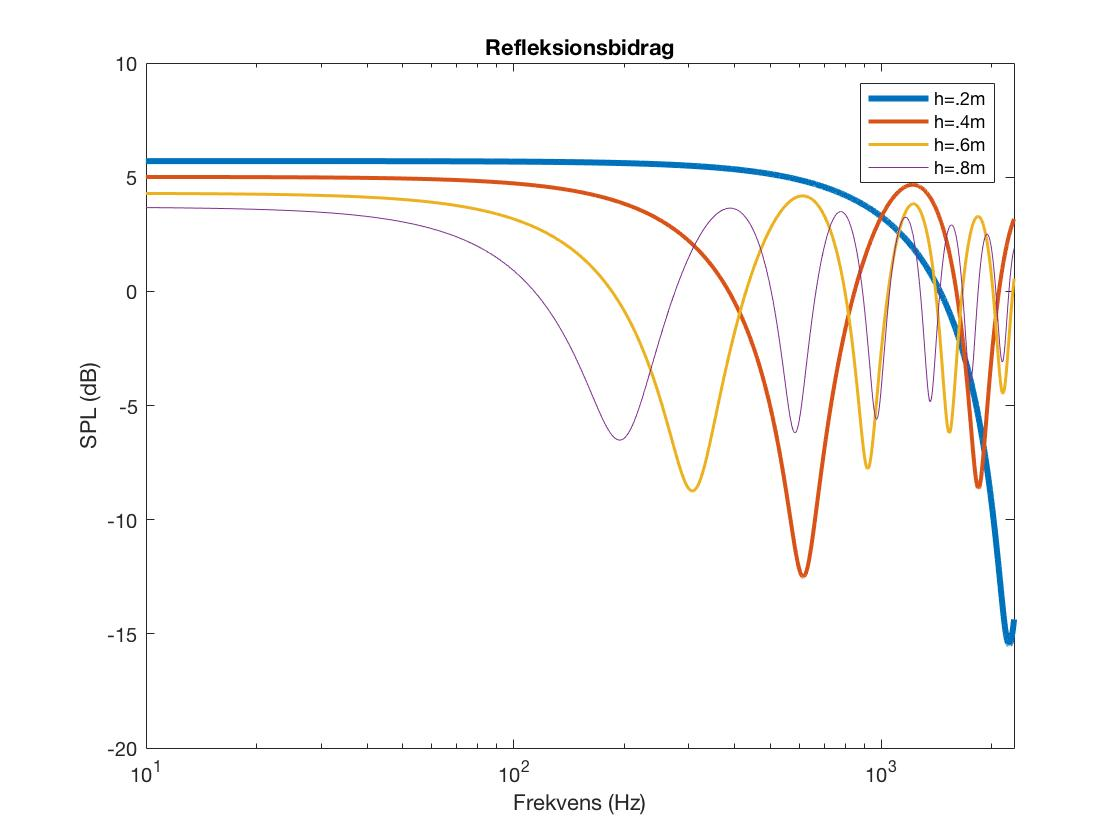
\includegraphics[width=\textwidth]{Pics/refleksionsbidrag}
	\caption{Refleksionsbidrag fra nærmeste hårde, reflekterende overflade til forskellige højder for højtaleren } 
	\label{fig:refleksionsbidrag}
\end{figure}

\section{Samlet Frekvensrespons}

Ved at kombinere bas-reflex kabinettets frekvensrespons, med det lavfrekvente gain for refleksionen ved nærtliggende overflader, opnås et frekvensrespons som kan ses i figur \ref{fig:sim_samletrespons}.

Af figuren fremgår det, at der er skabt et stabilt gain omkring 6dB i de lavere frekvenser under højtalerens resonansfrekvens, som bringer tidligere uhørbare frekvenser op i et lydtryk, hvor de rent faktisk kan opfattes af det menneskelige ører. Derudover, er de frekvenser som tidligere lå lige på grænsen af denne hørbarhed, løftet til et niveau hvor det burde være væsentligt lettere at høre.

Ulempen er desværre netop den destuktive interferens som skabes fra reflektionen, som ses på den blå kurve, tidligere omtalt i afsnit \ref{sec:reflection}.\\
Dette må dermed være et trade-off, imellem forstærkningen i de lave frekvenser og irregulariteten i de højere frekvenser. 

Det kan ydermere betragtes, at kurven aftager med 24dB/oktav under højtalerens resonansfrekvens, netop som teorien beskrev.\fixme{tores bog ref}
\begin{figure}[h!]
	\centering
	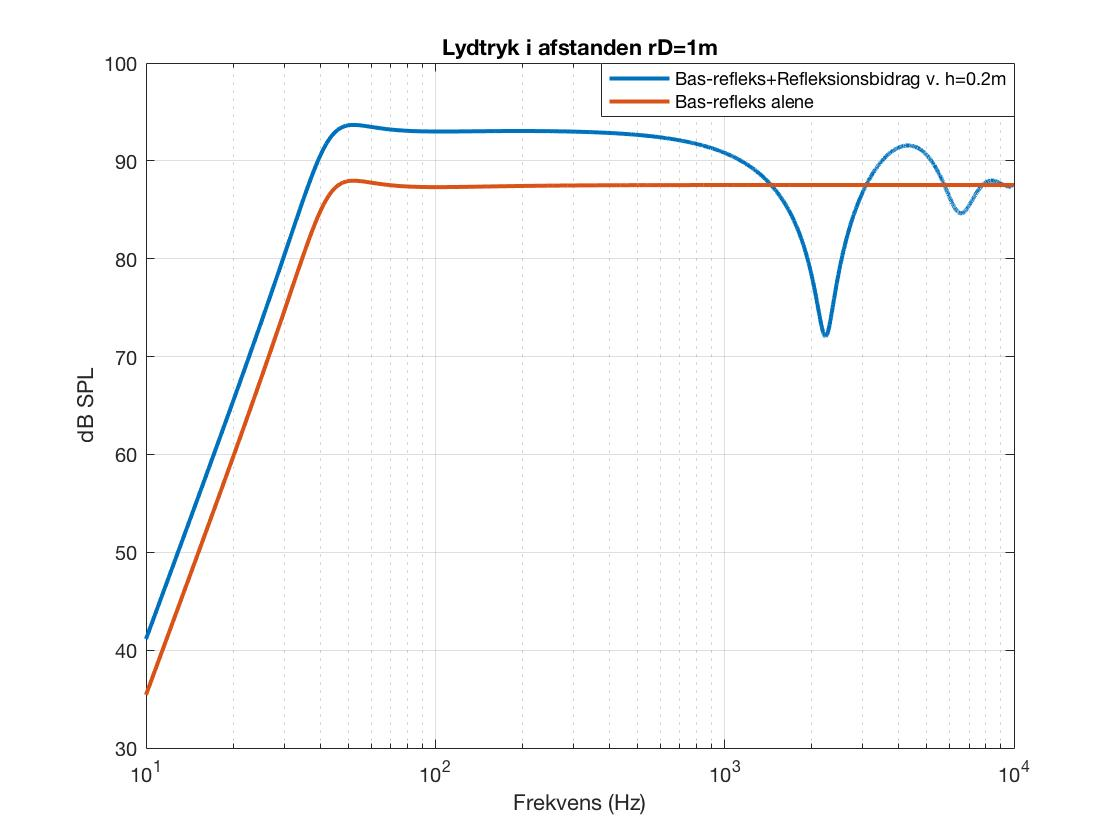
\includegraphics[width=\textwidth]{Pics/sim_samletrespons}
	\caption{Frekvensrespons for Basreflex-kabinettet med vs uden refleksionsbidraget} 
	\label{fig:sim_samletrespons}
\end{figure}



 
